\chapter{Mesure des inductances}

\section{Introduction}
La mesure présentée dans ce chapitre vise à redéfinir la valeur de l'inductance. Cette dernière étant considérée comme erronée à la suite des mesures précédentes, une nouvelle détermination a été réalisée au moyen d'un RLC-mètre. Cette démarche répond directement à l'hypothèse de la \autoref{sec:Hypothese} selon laquelle l'inductance nominale calculée est incorrecte.

\section{Protocole de mesure}
Afin de réaliser la mesure, les éléments suivants sont nécessaires :

\begin{itemize}
    \item Des cales de 1~mm, 1.5~mm, 2~mm et 3~mm (quatre exemplaires de chaque).
    \item Un RLC-mètre.
\end{itemize}

La mesure se réalise en plaçant les cales entre la partie lévitante et le profilé. Le RLC-mètre se branche directement sur les bornes des inducteurs.

\red{Important !} Il ne faut surtout pas alimenter la maquette lors de la mesure des inductances. Cela endommagerait l'appareil de mesure.

\section{Mesure des inductances}
La plage de mesure s'étend de 20~Hz à 25~kHz. Les mesures sont représentées de la \autoref{fig:MesInd1} à la \autoref{fig:MesInd4} :

\begin{figure}[H]
    \centering
    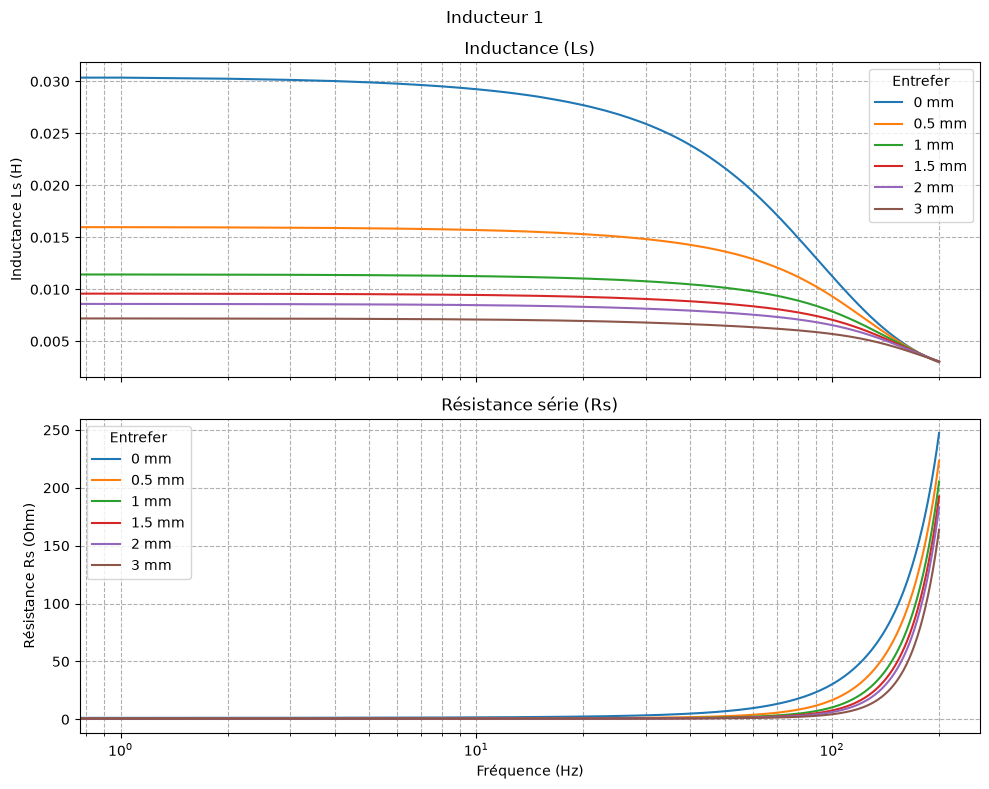
\includegraphics[width=0.85\linewidth]{assets/content/09-MesureInductance/MesInd1.png}
    \caption{Mesure sur l'inducteur 1}
    \label{fig:MesInd1}
\end{figure}

\begin{figure}[H]
    \centering
    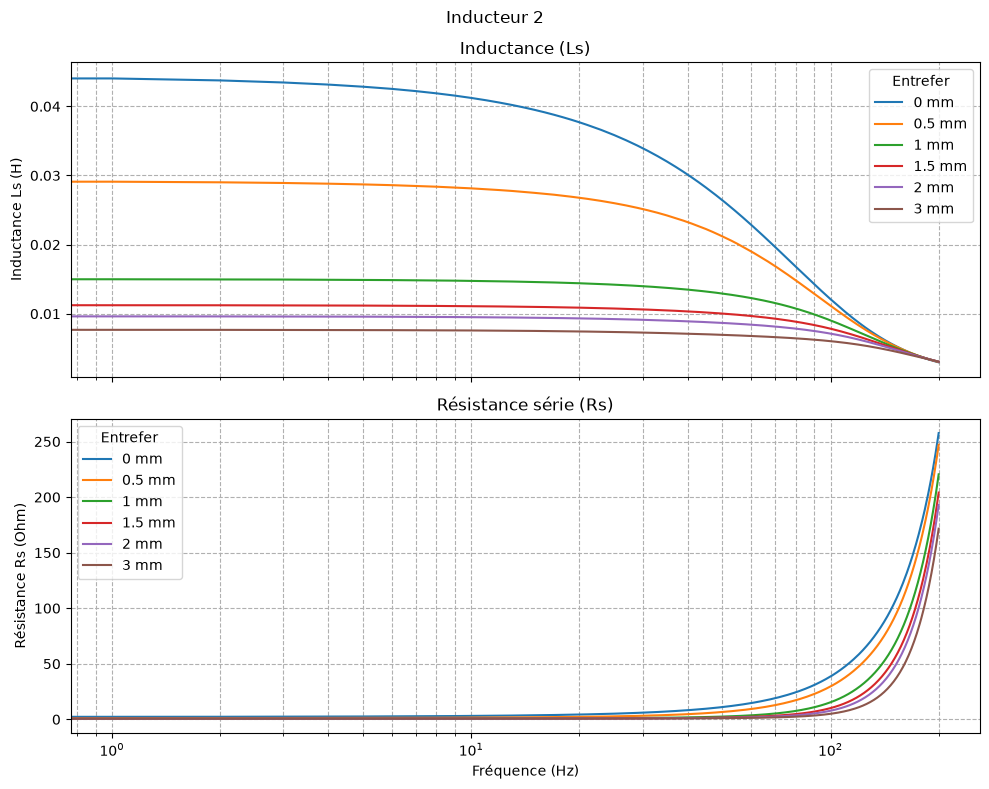
\includegraphics[width=0.9\linewidth]{assets/content/09-MesureInductance/MesInd2.png}
    \caption{Mesure sur l'inducteur 2}
    \label{fig:MesInd2}
\end{figure}

\begin{figure}[H]
    \centering
    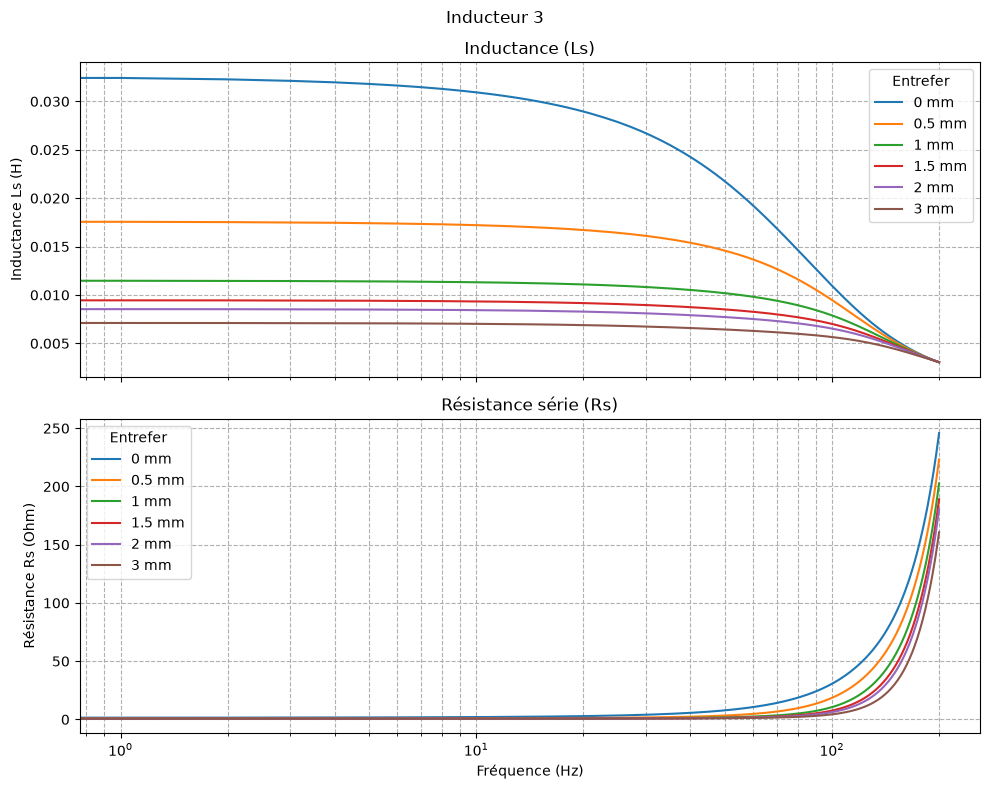
\includegraphics[width=0.9\linewidth]{assets/content/09-MesureInductance/MesInd3.png}
    \caption{Mesure sur l'inducteur 3}
    \label{fig:MesInd3}
\end{figure}

\begin{figure}[H]
    \centering
    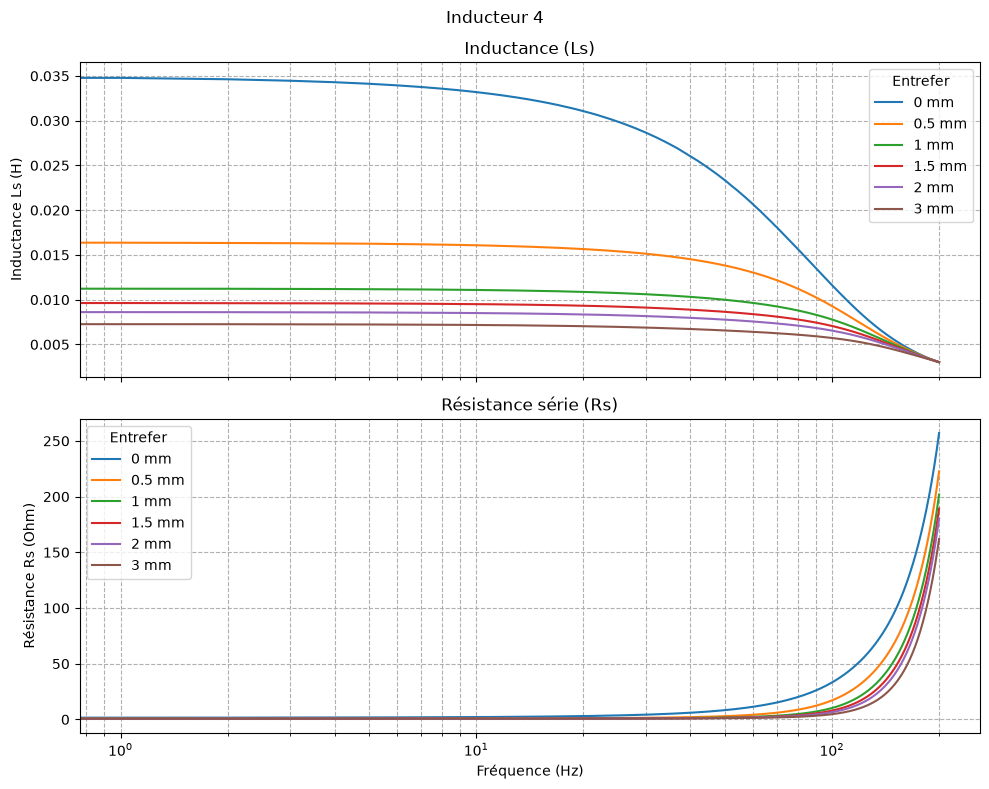
\includegraphics[width=0.9\linewidth]{assets/content/09-MesureInductance/MesInd4.png}
    \caption{Mesure sur l'inducteur 4}
    \label{fig:MesInd4}
\end{figure}

Une fréquence de lecture doit à présent être choisie afin d'y relever les paramètres de la bobine. Le point de lecture doit se situer en basse fréquence : du point de vue de la bobine, le courant issu de la PWM est similaire à celui d'une alimentation continue. La fréquence ne doit toutefois pas être choisie trop basse, afin d'éviter les bruits parasites provenant du RLC-mètre. De ce fait, les valeurs relevées à une fréquence de 120~Hz ont été sélectionnées. Ceci donne les valeurs suivantes :

\begin{table}[H]
    \centering
    \begin{tabular}{l ccc ccc cc}
        \toprule
        \textbf{Entrefer} & \textbf{Rs1}        & \textbf{Ls1}  & \textbf{Rs2}        & \textbf{Ls2}  & \textbf{Rs3}        & \textbf{Ls3}  & \textbf{Rs4}        & \textbf{Ls4}  \\
        \textbf{[mm]}     & \textbf{($\Omega$)} & \textbf{(mH)} & \textbf{($\Omega$)} & \textbf{(mH)} & \textbf{($\Omega$)} & \textbf{(mH)} & \textbf{($\Omega$)} & \textbf{(mH)} \\
        \midrule
        0                 & 7.24                & 21.44         & 11.37               & 26.06         & 8.04                & 21.48         & 8.62                & 23.06         \\
        0.5               & 2.82                & 13.57         & 6.85                & 20.99         & 3.42                & 14.49         & 3.02                & 13.75         \\
        1                 & 1.71                & 10.12         & 2.58                & 12.86         & 1.82                & 10.15         & 1.76                & 9.96          \\
        1.5               & 1.34                & 8.60          & 1.68                & 9.99          & 1.39                & 8.49          & 1.45                & 8.62          \\
        2                 & 1.17                & 7.74          & 1.37                & 8.65          & 1.23                & 7.70          & 1.34                & 7.75          \\
        3                 & 0.97                & 6.49          & 1.06                & 6.93          & 1.02                & 6.42          & 1.15                & 6.55          \\
        \bottomrule
    \end{tabular}
    \caption{Paramètres électriques en fonction de l'entrefer}
    \label{tab:mesures_entrefer}
\end{table}

\subsection{Analyse des mesures}
Comme observé, les inductances sont effectivement plus élevées. Au point nominal, soit un entrefer de 2~mm, les valeurs mesurées (comprises entre 7.7~mH et 8.65~mH) se rapprochent du double de la valeur théorique de 4.9~mH.

Ces valeurs peuvent s'expliquer par le fait que la surface effective de l'entrefer est en réalité plus grande que prévu, en raison des effets de bord du champ magnétique. Les calculs ont été réalisés une nouvelle fois en prenant en compte la réluctance du fer dans le calcul de l'inductance. Cependant, ces calculs n'ont pas apporté d'explication supplémentaire concernant ce doublement de la valeur.

Les valeurs mesurées seront par conséquent employées pour la synthèse de la régulation de courant ainsi que pour la méthode inverse. Celles retenues correspondent au point nominal, soit un entrefer de 2~mm. Ces valeurs sont représentées dans le \autoref{tab:mesures_2mm} :

\begin{table}[H]
    \centering
    \begin{tabular}{l ccc ccc cc}
        \toprule
        \textbf{Entrefer} & \textbf{Rs1}        & \textbf{Ls1}  & \textbf{Rs2}        & \textbf{Ls2}  & \textbf{Rs3}        & \textbf{Ls3}  & \textbf{Rs4}        & \textbf{Ls4}  \\
        \textbf{[mm]}     & \textbf{($\Omega$)} & \textbf{(mH)} & \textbf{($\Omega$)} & \textbf{(mH)} & \textbf{($\Omega$)} & \textbf{(mH)} & \textbf{($\Omega$)} & \textbf{(mH)} \\
        \midrule
        2                 & 1.17                & 7.74          & 1.37                & 8.65          & 1.23                & 7.70          & 1.34                & 7.75          \\
        \bottomrule
    \end{tabular}
    \caption{Valeurs retenues pour un entrefer de 2~mm}
    \label{tab:mesures_2mm}
\end{table}

\section{Mesure du comportement du système}
Une fois les nouvelles valeurs d'inductance déterminées, le comportement du système a été analysé une nouvelle fois afin d'observer la différence. Les modifications suivantes ont été apportées :

\begin{enumerate}
    \item Implémentation des quatre valeurs d'inductance.
    \item Implémentation de quatre constantes pour le calcul du courant.
    \item Implémentation de quatre forces maximales utilisées pour l'anti-windup.
\end{enumerate}

Cela donne dès lors les définitions suivantes :

\begin{minted}{c}
// Inductance nominal au point nominal
#define L_N1            ((float)7.742e-3)
#define L_N2            ((float)8.647e-3)
#define L_N3            ((float)7.699e-3)
#define L_N4            ((float)7.750e-3)
...
#define K_FC1            ((float)(2.0/(L_N1*DELTA_N)))
#define K_FC2            ((float)(2.0/(L_N2*DELTA_N)))
#define K_FC3            ((float)(2.0/(L_N3*DELTA_N)))
#define K_FC4            ((float)(2.0/(L_N4*DELTA_N)))
...
#define FMAX1           ((float)(0.5*L_N1*DELTA_N*(IMAX/DELTA_0)*(IMAX/DELTA_0)))
#define FMAX2           ((float)(0.5*L_N2*DELTA_N*(IMAX/DELTA_0)*(IMAX/DELTA_0)))
#define FMAX3           ((float)(0.5*L_N3*DELTA_N*(IMAX/DELTA_0)*(IMAX/DELTA_0)))
#define FMAX4           ((float)(0.5*L_N4*DELTA_N*(IMAX/DELTA_0)*(IMAX/DELTA_0)))
\end{minted}

La mesure se réalise en se basant sur la méthode détaillée dans l'\autoref{annexe:MethodeMesurePosition}.

La mesure étant réalisée sur une période bien plus longue, la mesure complète est disponible dans l'\autoref{annexe:MesureComplete}. Les résultats présentés ici se concentrent sur une fenêtre de 10~s, comme illustré de la \autoref{fig:AnalyseInd1} à la \autoref{fig:AnalyseInd4} :

\begin{figure}[H]
    \centering
    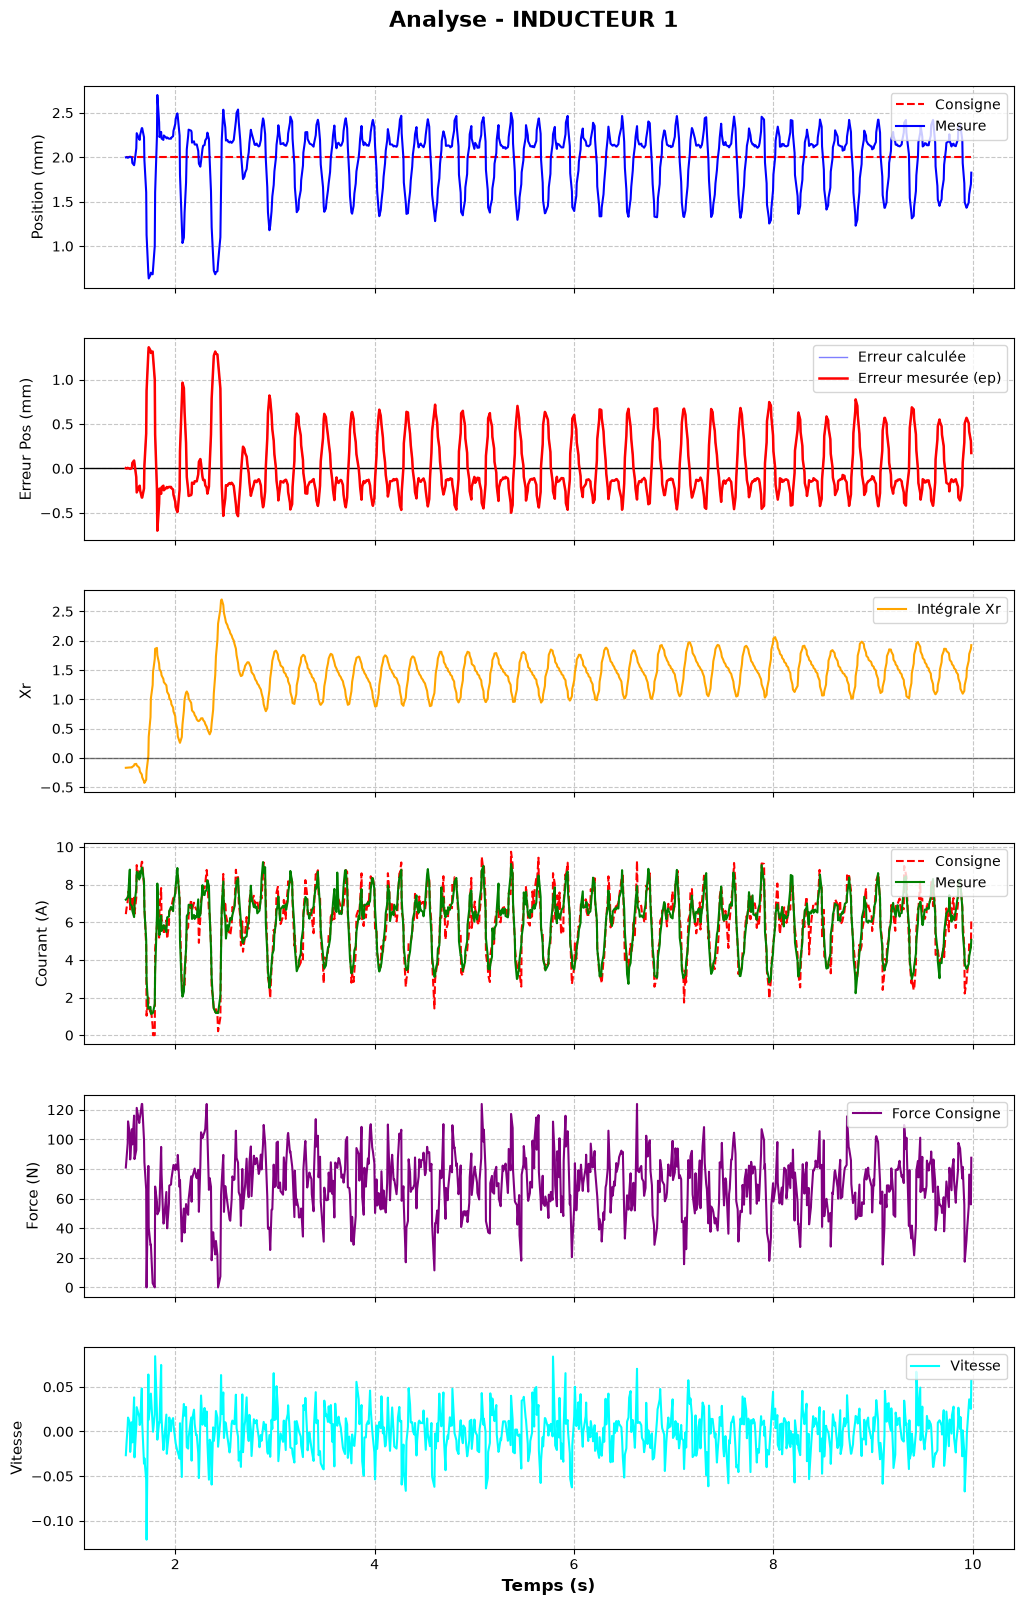
\includegraphics[width=1\linewidth]{assets/content/09-MesureInductance/AnalyseInd1.png}
    \caption{Mesure sur 10~s de la régulation de position sur l'inducteur 1}
    \label{fig:AnalyseInd1}
\end{figure}

\begin{figure}[H]
    \centering
    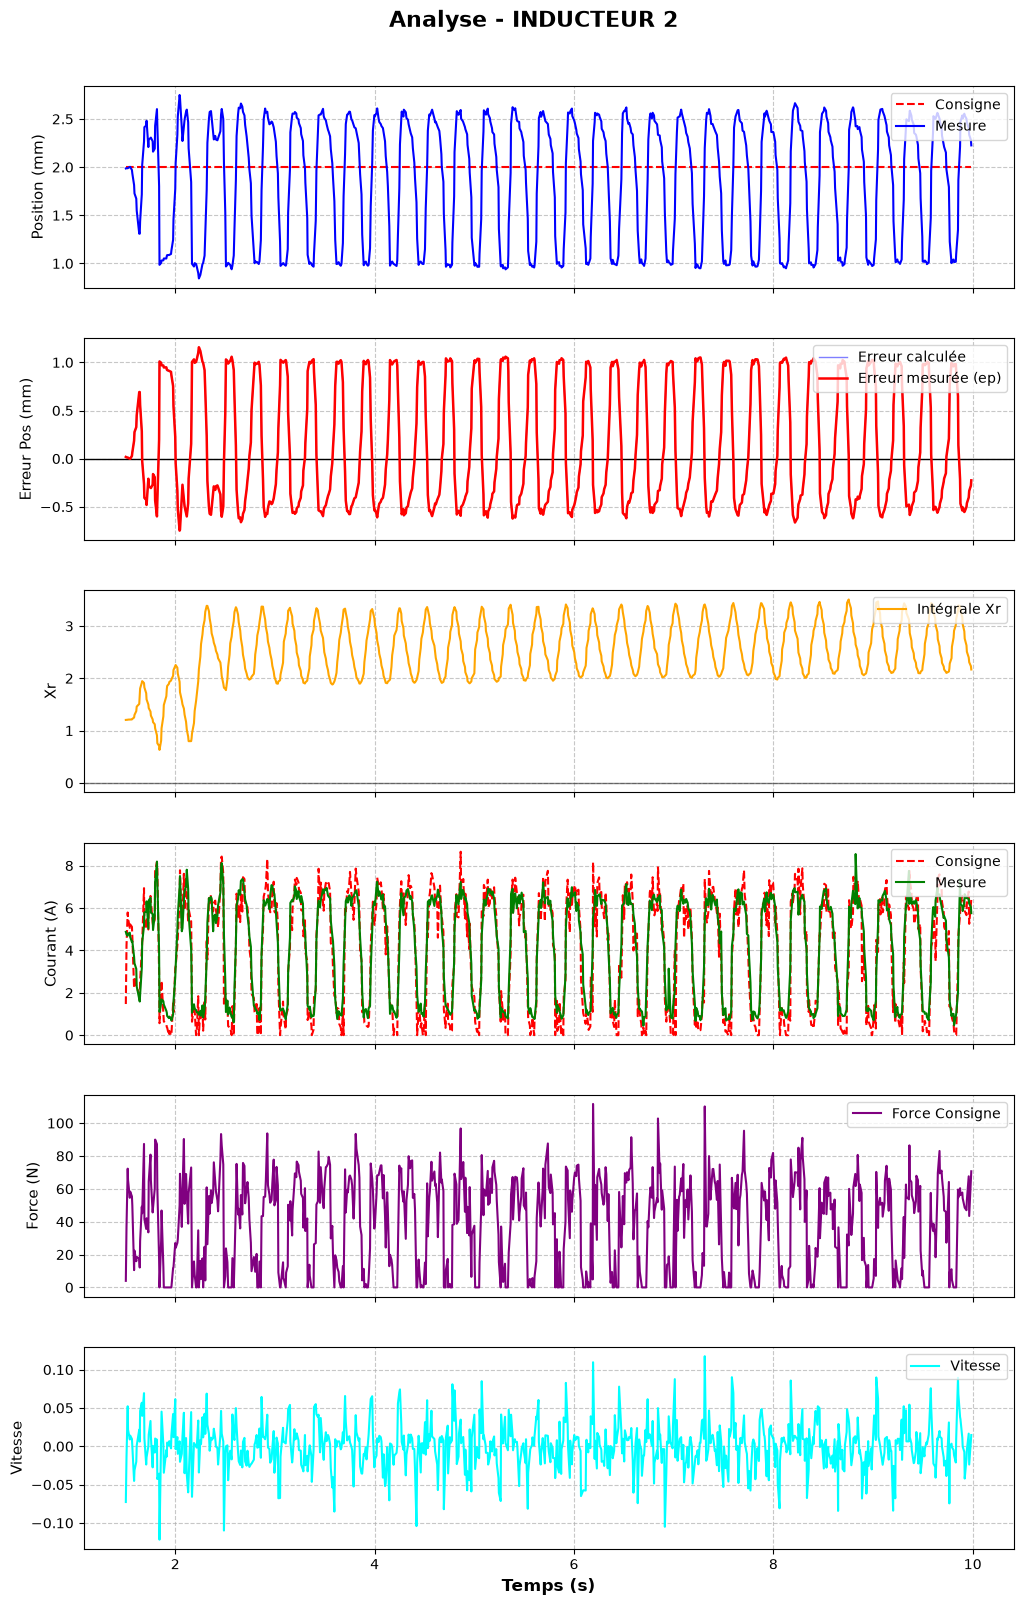
\includegraphics[width=1\linewidth]{assets/content/09-MesureInductance/AnalyseInd2.png}
    \caption{Mesure sur 10~s de la régulation de position sur l'inducteur 2}
    \label{fig:AnalyseInd2}
\end{figure}

\begin{figure}[H]
    \centering
    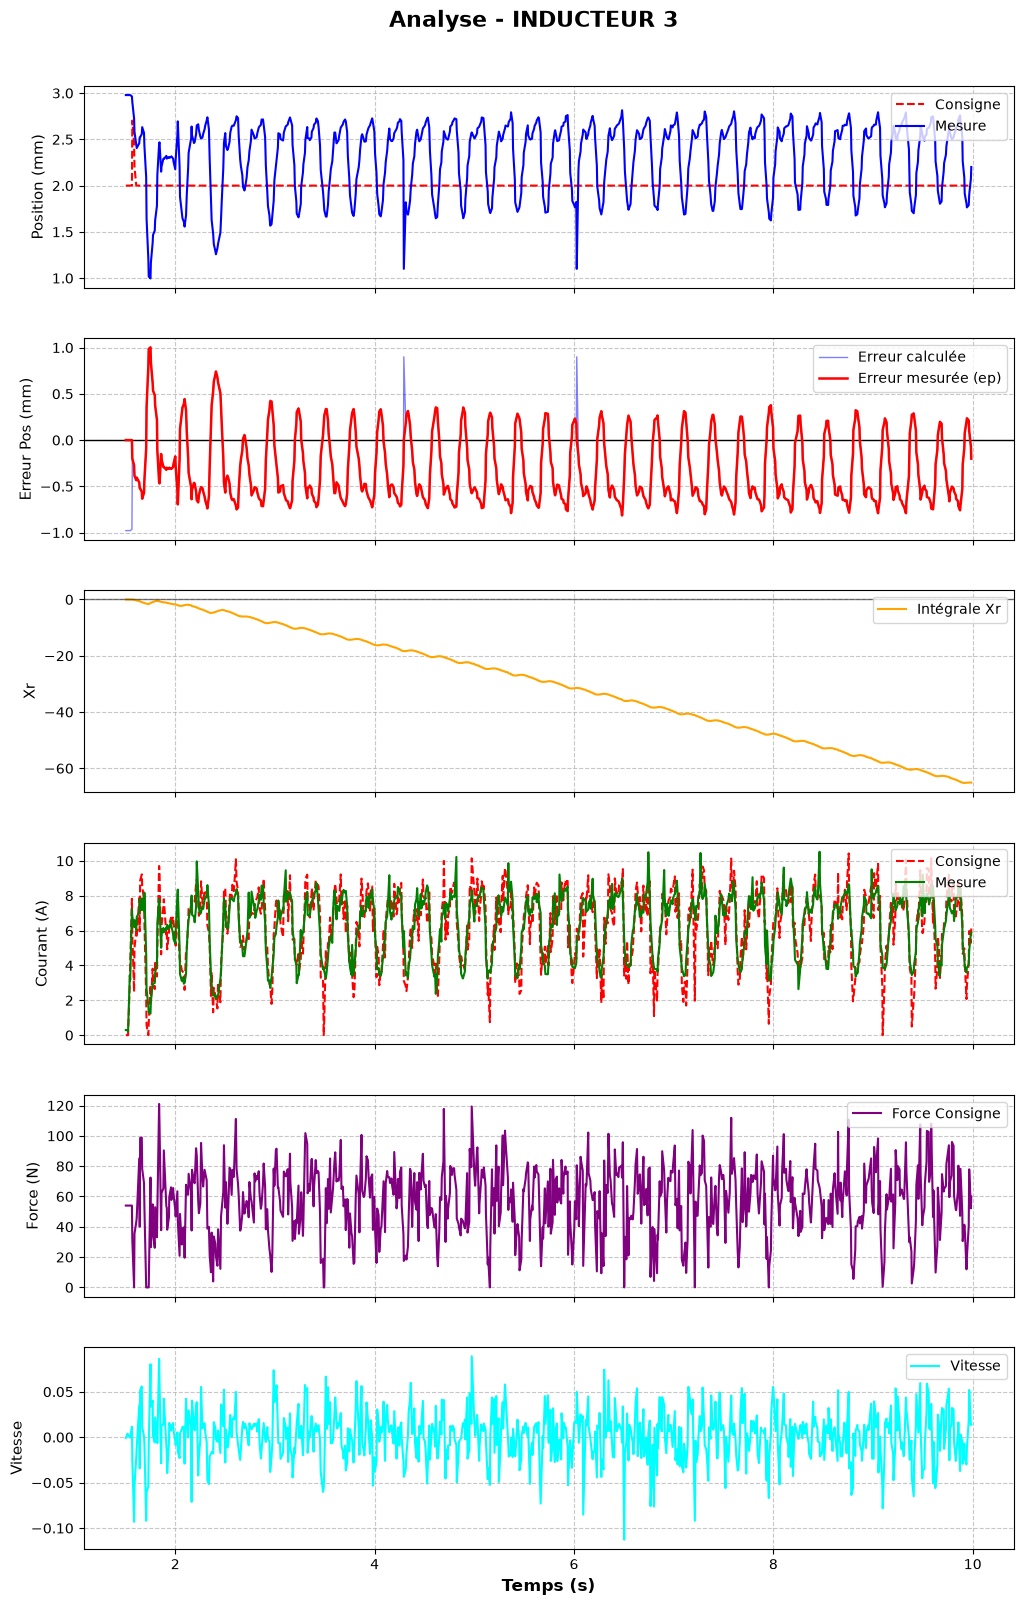
\includegraphics[width=1\linewidth]{assets/content/09-MesureInductance/AnalyseInd3.png}
    \caption{Mesure sur 10~s de la régulation de position sur l'inducteur 3}
    \label{fig:AnalyseInd3}
\end{figure}

\begin{figure}[H]
    \centering
    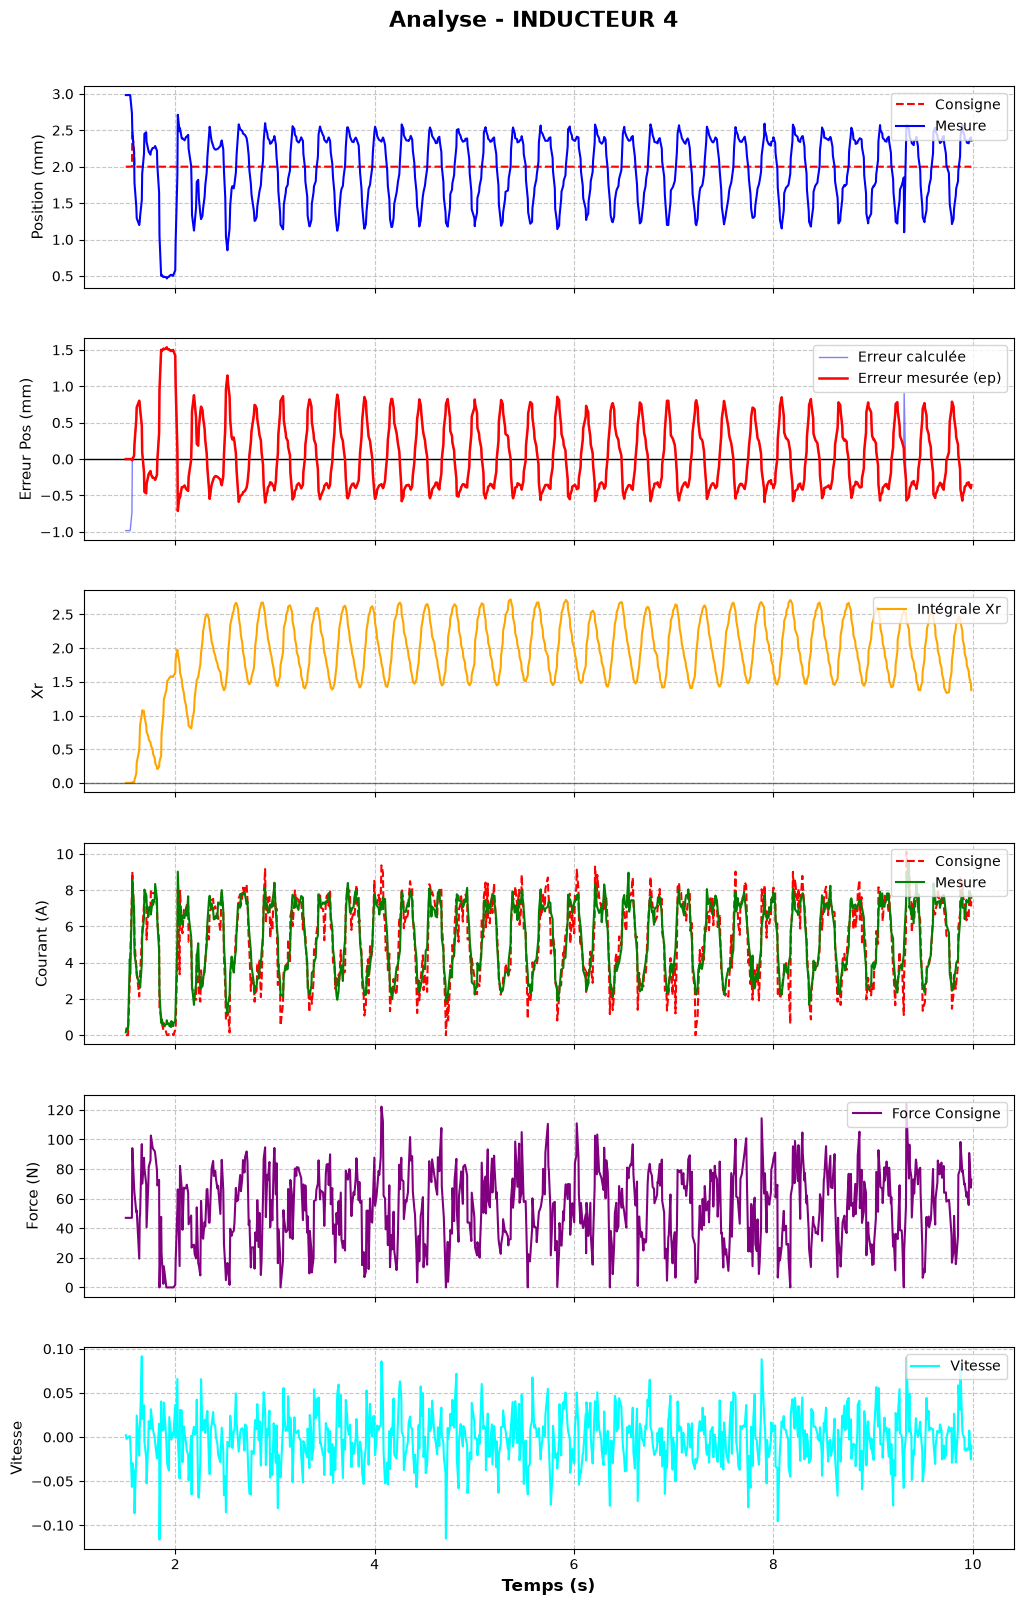
\includegraphics[width=1\linewidth]{assets/content/09-MesureInductance/AnalyseInd4.png}
    \caption{Mesure sur 10~s de la régulation de position sur l'inducteur 4}
    \label{fig:AnalyseInd4}
\end{figure}

Une fois cela fait, il est possible de réaliser une analyse des forces, comme dans la \autoref{fig:AnalyseForce} :

\begin{figure}[H]
    \centering
    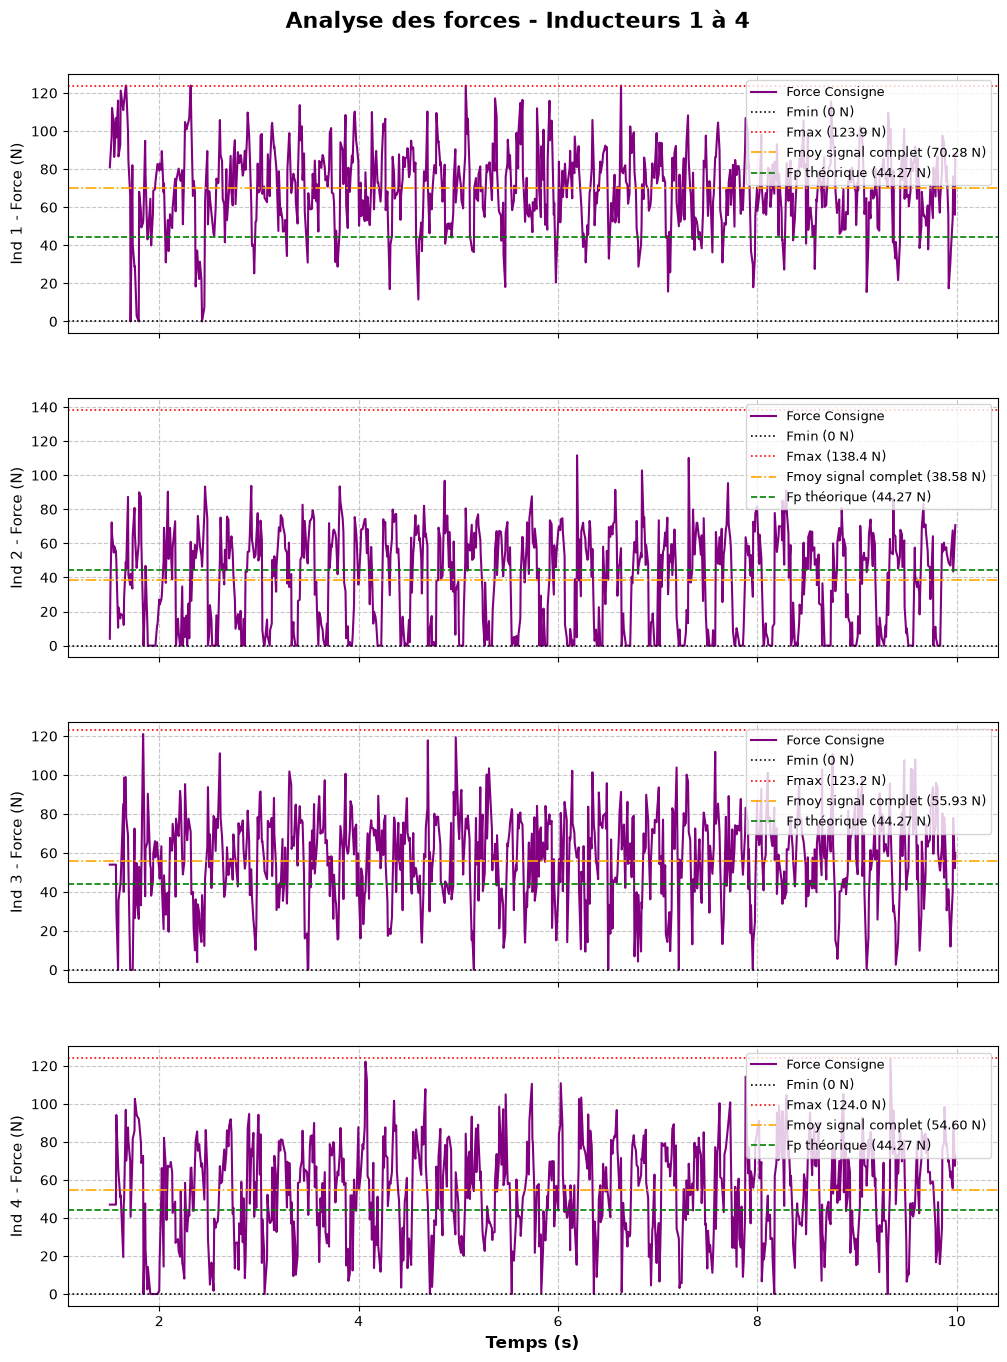
\includegraphics[width=0.9\linewidth]{assets/content/09-MesureInductance/AnalyseForce.png}
    \caption{Analyse des forces mesurées par inducteur}
    \label{fig:AnalyseForce}
\end{figure}

Il est alors possible de calculer les écarts présentés dans le \autoref{tab:forces_inducteurs_v2} :

\begin{table}[H]
    \centering
    \begin{tabular}{l cccc}
        \toprule
        \textbf{Inducteur} & \textbf{$F_{\text{moy}}$ mesurée [N]} & \textbf{$F_p$ théorique [N]} & \textbf{Écart [N]} & \textbf{Écart relatif [\%]} \\
        \midrule
        Inducteur 1        & 70.28                                 & 44.27                        & 26.01              & 58.74                       \\
        Inducteur 2        & 38.58                                 & 44.27                        & -5.70              & -12.87                      \\
        Inducteur 3        & 55.94                                 & 44.27                        & 11.66              & 26.34                       \\
        Inducteur 4        & 54.61                                 & 44.27                        & 10.33              & 23.34                       \\
        \bottomrule
    \end{tabular}
    \caption{Comparaison des forces moyennes mesurées et théoriques par inducteur}
    \label{tab:forces_inducteurs_v2}
\end{table}

\section{Analyse des résultats}
Comme constaté une nouvelle fois, la force mesurée s'écarte encore de la valeur théorique supposée. En fonctionnement complet (quatre inducteurs), il est possible de constater que le système oscille énormément. Cela rejoint l'une des explications précédentes : les inducteurs agissent l'un sur l'autre, empêchant chacun d'obtenir une stabilité.

La régulation de position sera dès lors modifiée afin de ne plus réaliser une régulation par inducteur (système en SISO), mais une régulation de position dans l'espace (système en MIMO).

La composante intégrale de l'inducteur 3 présente une pente descendante ; cela est dû au fait que son action intégrale a été retirée.

\section{Conclusion}
La mesure de l'inductance a démontré que les valeurs d'inductance sont effectivement supérieures à celle calculée. L'hypothèse de la \autoref{sec:Hypothese} selon laquelle l'inductance nominale calculée est incorrecte est donc confirmée. Il sera dès lors possible d'employer ces valeurs mesurées afin d'améliorer l'état actuel de la maquette, notamment pour la synthèse de la régulation de courant et la méthode inverse.

La seconde mesure indique une nouvelle fois une instabilité de la régulation de position. Une approche différente sera dès lors adoptée pour réaliser la régulation, celle-ci montrant ses limites.